% ============================================================
% Chapitre 3 : Conception
% ============================================================
\chapter{Conception}

\begin{spacing}{1.2}
\minitoc
\thispagestyle{MyStyle}
\end{spacing}
\newpage

\section*{Introduction}

Le chapitre précédent a établi ce que le système doit faire. Celui ci décrit comment il est construit pour le faire. Nous présentons d'abord la vue statique, c'est à dire l'organisation des éléments qui composent la plateforme et les relations qu'ils entretiennent, puis sa vue dynamique, c'est à dire la manière dont ces éléments collaborent dans le temps. Nous détaillons ensuite la conception de la couche agentique, qui constitue l'apport principal de ce travail, et celle du contrôle d'accès, qui en conditionne la sûreté. Conformément à l'usage, cette partie reste indépendante des technologies employées : celles ci sont introduites au chapitre suivant.

\section{Vue statique de l'application}

\subsection{Architecture logique du logiciel}

\subsubsection{Le principe retenu}

L'architecture repose sur une séparation en couches concentriques, selon le patron dit hexagonal, également appelé architecture en ports et adaptateurs \cite{cockburn, martin}. Ce choix découle directement de deux besoins non fonctionnels établis au chapitre précédent. L'extensibilité exige qu'un changement de fournisseur externe ne se propage pas dans le système ; la testabilité exige que la logique de décision puisse être vérifiée sans dépendre d'un environnement.

Le principe est le suivant. Au centre se trouve le domaine métier, qui contient les entités, les objets valeur et les règles. Ce domaine ne dépend de rien : il ignore par construction l'existence des interfaces utilisateur, des bases de données, des fournisseurs de reconnaissance vocale et des systèmes de l'opérateur. Il déclare en revanche des interfaces abstraites, appelées ports, qui expriment ce dont il a besoin sans dire comment le lui fournir. Autour de ce centre viennent les adaptateurs, qui implémentent ces ports en s'adressant au monde extérieur.

La conséquence pratique est que la direction des dépendances est inversée par rapport à une organisation en couches classique. Ce n'est pas le domaine qui dépend de l'infrastructure, c'est l'infrastructure qui se conforme au contrat défini par le domaine. Remplacer un fournisseur revient alors à écrire un nouvel adaptateur, sans toucher ni aux règles ni aux entités.

La figure \ref{fig:archi-hexagonale} présente cette organisation.

\figureTikz{Architecture hexagonale de la plateforme}{archi-hexagonale}{fig-archi-hexagonale}

\subsubsection{Les ports du domaine}

Le domaine déclare treize ports, chacun correspondant à une capacité dont il a besoin et dont il refuse de connaître la réalisation. Le tableau \ref{tab:ports} les récapitule.

\begin{table}[H]
\centering
\renewcommand{\arraystretch}{1.2}
\begin{tabular}{|p{3.0cm}|p{11.5cm}|}
\hline
\textbf{Port} & \textbf{Capacité déclarée} \\
\hline
Décision & Proposer une action candidate assortie d'un degré de confiance. \\
\hline
Politique & Rendre un verdict motivé sur une action, et contrôler une réponse sortante. \\
\hline
Exécution & Réaliser une action approuvée de manière idempotente. \\
\hline
Connaissance & Rechercher les passages documentaires pertinents pour une question. \\
\hline
Audit & Inscrire un enregistrement infalsifiable et en vérifier la chaîne. \\
\hline
Notification & Acheminer un avis vers un client ou un conseiller. \\
\hline
Gestion de tickets & Créer, consulter, mettre à jour et clôturer un ticket. \\
\hline
Relation client & Accéder au profil et à la situation contractuelle d'un client. \\
\hline
Facturation & Consulter les factures et les montants dus. \\
\hline
Solde & Consulter et créditer le solde d'une ligne. \\
\hline
Paiement & Réaliser une opération de règlement. \\
\hline
Supervision réseau & Consulter l'état du réseau et les incidents en cours. \\
\hline
Provisionnement & Agir sur la configuration d'une ligne ou d'une carte SIM. \\
\hline
\end{tabular}
\caption{Ports déclarés par le domaine métier}
\label{tab:ports}
\end{table}

Le port de politique mérite une remarque particulière, car il déclare deux capacités et non une seule. La première évalue une action avant son exécution. La seconde évalue une réponse avant son émission, ce qui permet de contrôler ce que le système s'apprête à dire au client, et non uniquement ce qu'il s'apprête à faire. Cette symétrie est délibérée : une réponse qui divulguerait une donnée personnelle ou formulerait un engagement non fondé constitue un incident au même titre qu'une action non autorisée.

\subsubsection{Découpage en contextes métier}

Le domaine n'est pas monolithique. Il est découpé en contextes métier délimités, au sens de la conception pilotée par le domaine \cite{evans}. Chacun possède son propre vocabulaire et sa propre logique, et communique avec les autres par des contrats explicites plutôt que par des structures partagées. Ce découpage suit les frontières du métier et non celles de la technique.

\begin{itemize}
  \item \textbf{Conversation.} Le déroulement de l'échange, les tours de parole, l'état de la session et l'issue de la conversation.
  \item \textbf{Connaissance.} Les documents, leurs versions, leurs fragments et leur indexation.
  \item \textbf{Décision et politique.} La proposition d'action, les règles métier et les verdicts rendus.
  \item \textbf{Exécution.} Le registre des actions, leur identité d'opération et leur statut.
  \item \textbf{Gestion de tickets.} Les tickets et leur cycle de vie.
  \item \textbf{Routage et escalade.} Les conseillers, leurs disponibilités, les rappels et les dossiers d'escalade.
  \item \textbf{Identité et accès.} Les comptes du portail, les sessions et les droits.
  \item \textbf{Audit.} La chaîne des enregistrements et sa vérification.
  \item \textbf{Référentiels.} Les catalogues de produits, de recharges, de zones géographiques et de règles.
\end{itemize}

La figure \ref{fig:paquetages} présente ce découpage sous forme de diagramme de paquetages, en faisant apparaître les dépendances autorisées entre contextes.

\figureTikz{Diagramme de paquetages des contextes métier}{paquetages}{fig-paquetages}

\subsubsection{Décomposition en composants}

À l'exécution, ces contextes se matérialisent sous forme de composants déployables indépendants. Chacun expose une interface de service et n'accède aux autres qu'au travers de celle ci, ce qui garantit que le découpage logique survit au passage à l'exécution. La figure \ref{fig:composants} présente cette décomposition.

\figureTikz{Diagramme de composants de la plateforme}{composants}{fig-composants}

Trois règles de construction gouvernent cette décomposition et méritent d'être énoncées, car elles conditionnent la validité de l'ensemble.

\begin{itemize}
  \item Les règles métier n'importent aucune bibliothèque de fournisseur. Elles se situent derrière les ports et ignorent l'existence des fournisseurs externes.
  \item Le point d'entrée de la couche temps réel n'est qu'un assembleur. Il compose les éléments entre eux et ne contient aucune logique métier.
  \item Les capacités offertes à la couche conversationnelle sont des façades minces. Elles n'implémentent rien : elles appellent les services du domaine au travers d'interfaces typées.
\end{itemize}

Ces trois règles servent un objectif unique. Elles garantissent qu'aucun chemin ne permet d'atteindre une action métier en contournant les contrôles, parce que le seul chemin qui existe passe par le domaine.

\subsection{Diagrammes de classes}

Nous présentons trois diagrammes de classes, chacun répondant à une question distincte. Le premier décrit le modèle du domaine. Le deuxième décrit la couche des agents conversationnels. Le troisième décrit le moteur de décision déterministe.

\subsubsection{Modèle du domaine}

Le modèle du domaine distingue explicitement deux natures d'objets, distinction qui structure l'ensemble du code.

Les entités possèdent une identité propre qui persiste au delà de leurs valeurs : deux clients restent distincts même si tous leurs attributs coïncident. Le domaine s'organise autour de cinq racines d'agrégat — le client, la conversation, le dossier d'assistance, l'opération et la règle métier — auxquelles se rattachent les entités qui leur appartiennent : l'abonnement et le compte pour le client, le tour de parole et l'intention pour la conversation, le ticket, l'affectation et le conseiller pour l'assistance, la décision d'autorisation pour l'opération, et l'entrée d'audit, qui consigne chaque acte. L'opération et la règle métier sont par ailleurs abstraites : la première est déclinée en paiement de facture, réclamation et gestion d'abonnement, la seconde en règles de seuil et de niveau de vérification.

Les objets valeur, au contraire, n'ont pas d'identité : ils sont définis entièrement par leur contenu et sont immuables. Le domaine en distingue quatre, et le choix de chacun d'eux est significatif. Le numéro d'appel encapsule sa propre règle de validité, ce qui rend impossible la circulation d'un numéro mal formé dans le système. Le montant transporte indissociablement sa valeur et sa devise, ce qui interdit une addition entre devises différentes. L'identité d'opération est la clé qui garantit qu'une action ne sera pas exécutée deux fois. Le créneau, enfin, borne un intervalle de rappel réel proposé au client.

Le domaine définit également de nombreuses énumérations qui ferment les ensembles de valeurs admissibles : les langues prises en charge, les canaux de communication, le locuteur, le sentiment, le motif de clôture, la décision du moteur, le statut de l'opération, le motif d'escalade, le mode d'assistance, la priorité et l'état du ticket. Fermer ces ensembles n'est pas un détail de style. Une valeur inattendue devient une erreur détectable à la frontière du système plutôt qu'un comportement silencieux en son coeur.

La figure \ref{fig:classes-domaine} présente ce modèle.

\begin{figure}[htbp]
    \centering
    \setlength{\fboxsep}{0pt}
    \setlength{\fboxrule}{1pt}
    \fbox{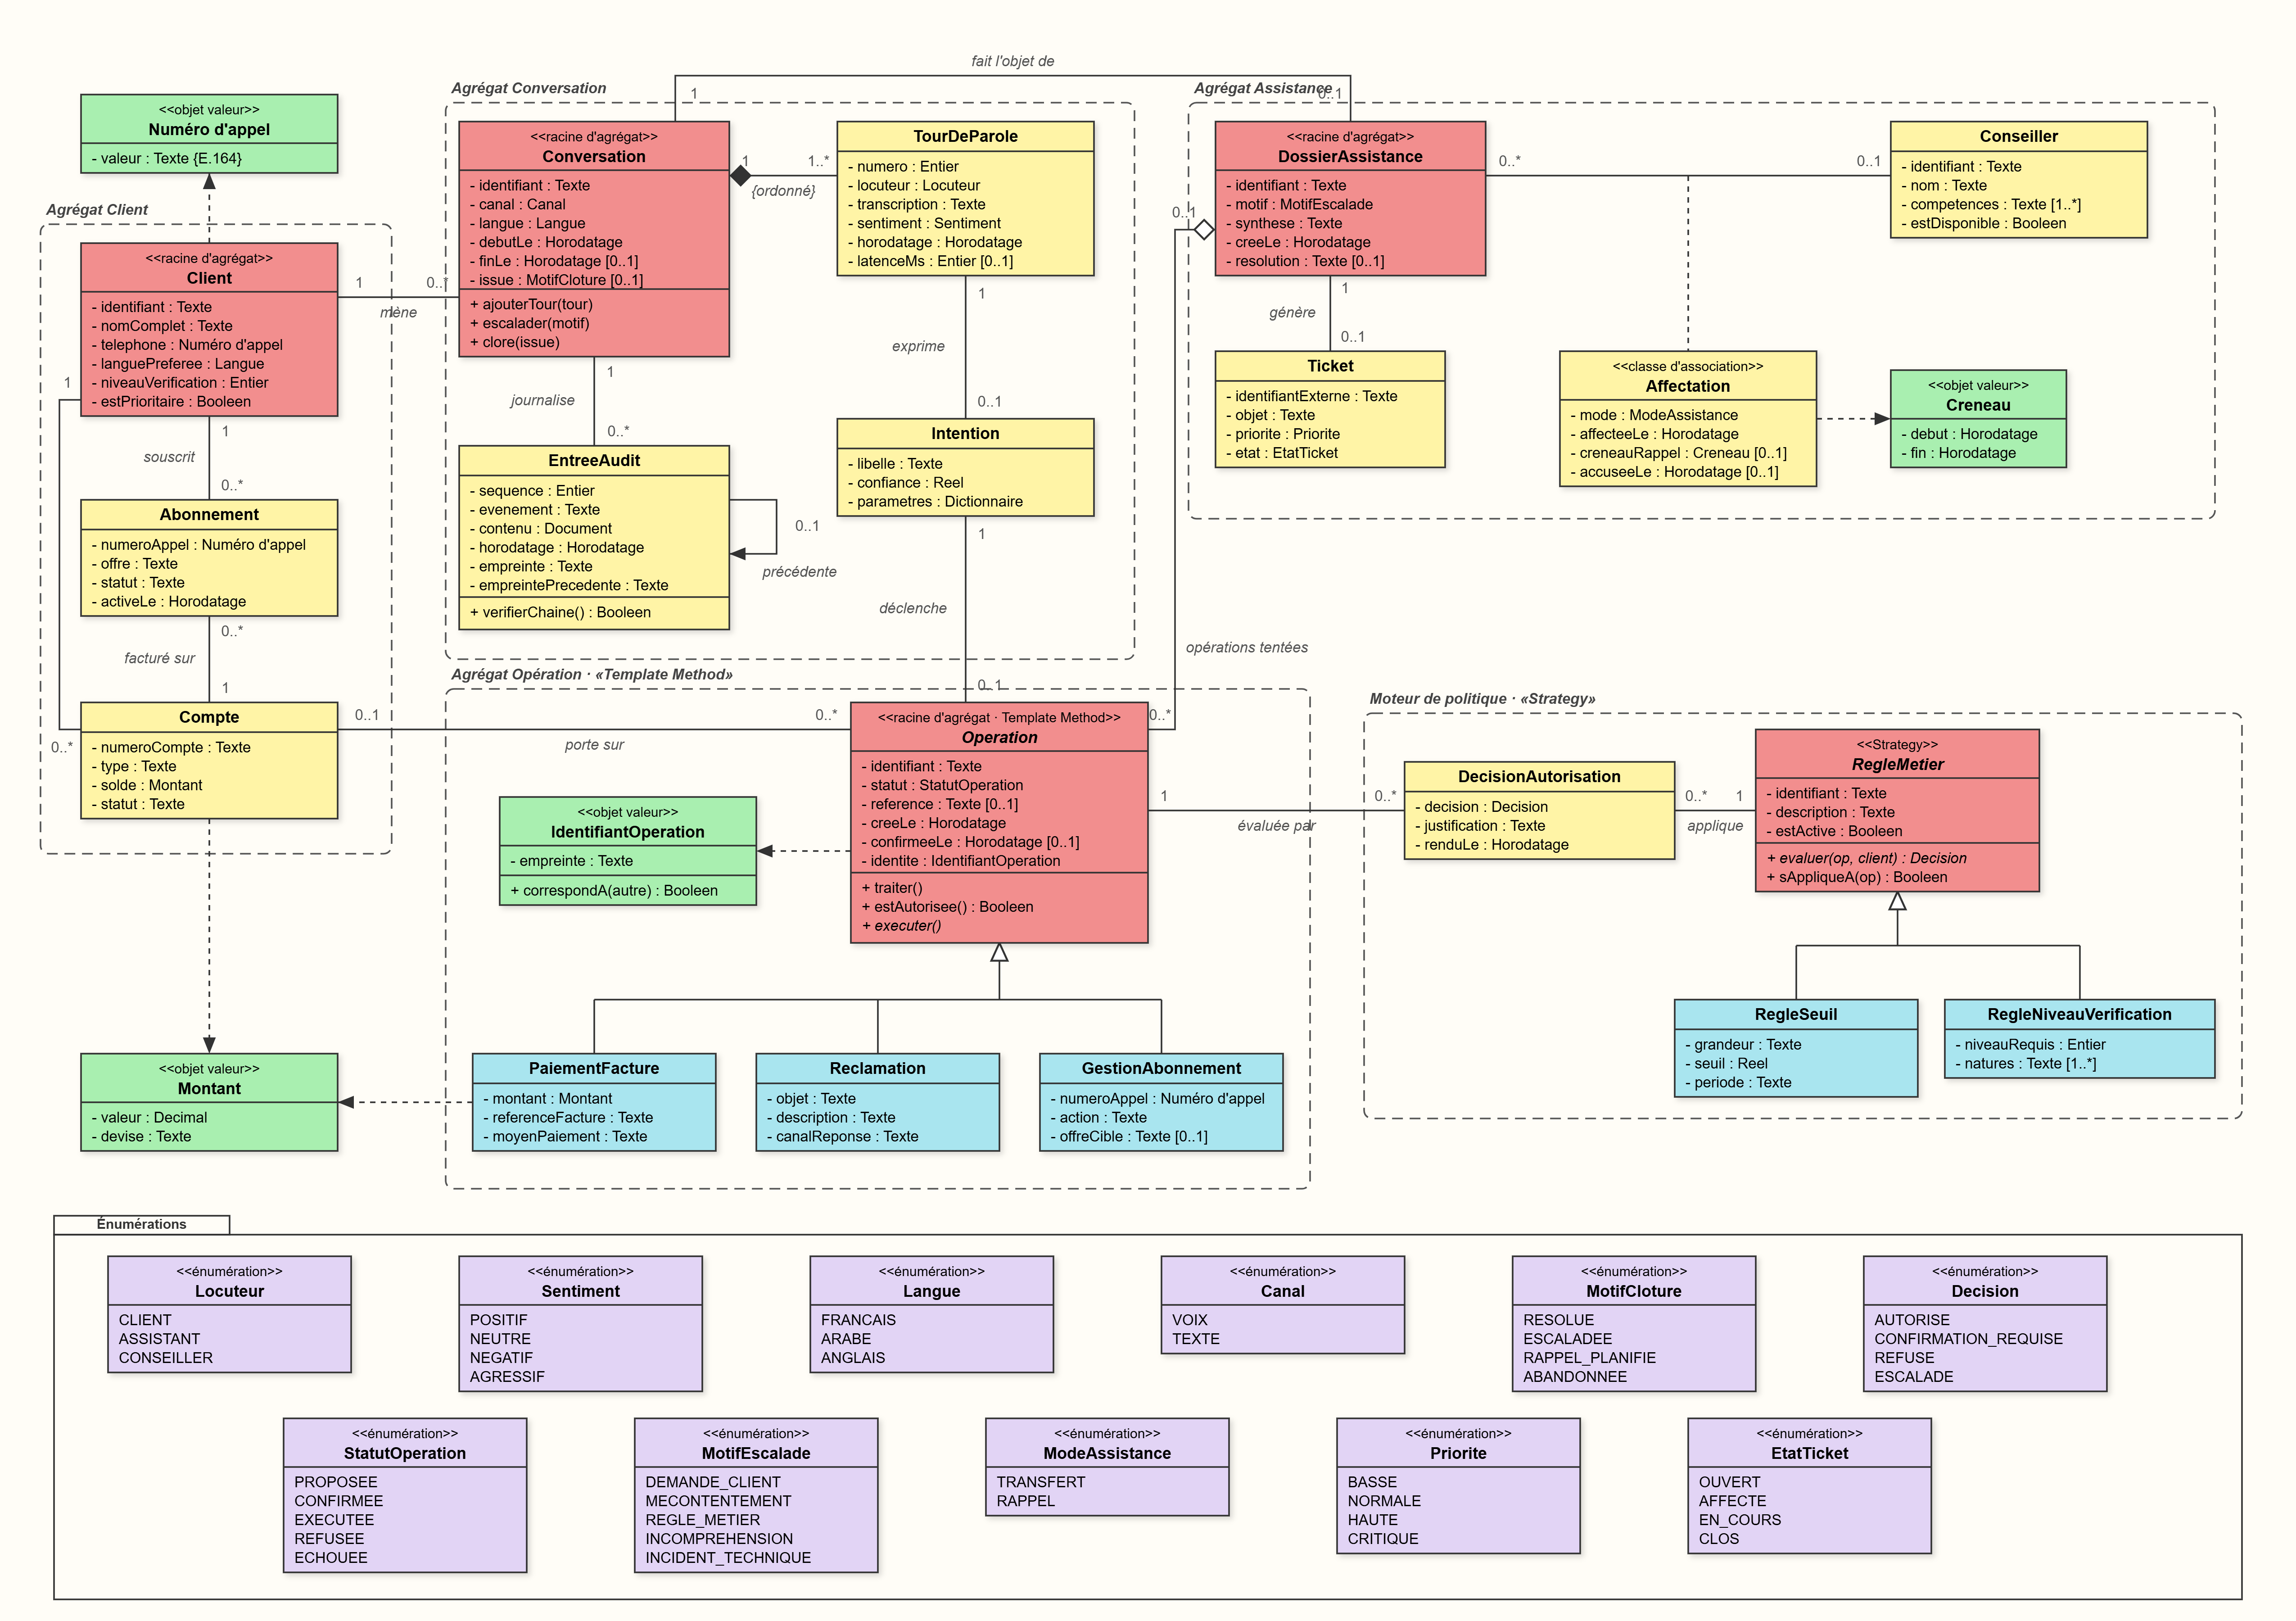
\includegraphics[width=\linewidth, height=0.82\textheight, keepaspectratio]{figures/fig-classes-domaine.png}}
    \vspace{0.2cm}
    \caption{Diagramme de classes du modèle du domaine}
    \label{fig:classes-domaine}
\end{figure}

\subsubsection{Couche des agents conversationnels}

La couche conversationnelle ne tient pas dans une simple hiérarchie : quatre classes d'orchestration en constituent la colonne vertébrale. La session vocale pilote le pipeline vocal, journalise l'échange dans la conversation, applique les règles de session, compose le contexte de session et détient l'agent actif. Le registre des agents agrège les agents et compose les définitions de domaine ; il sait renvoyer l'agent initial, l'agent d'un domaine ou celui qui correspond à une intention. Le générateur d'instructions compose les instructions d'un agent à partir de sa définition de domaine, de ses outils et de la langue, puis les adapte au contexte. Les règles de session bornent enfin l'ensemble : nombre maximal de transferts et de clarifications, seuil de mécontentement, autorisation d'un transfert, exigence d'une clarification ou d'une escalade.

Les agents proprement dits forment une hiérarchie à deux niveaux. \emph{AgentDeBase} porte le domaine, les instructions et les comportements communs — se présenter, traiter un tour, déterminer si une intention relève de son périmètre, exposer ses outils spécifiques, demander un transfert, journaliser le tour. Cinq agents en dérivent, et la généralisation porte la contrainte \{disjoint, complet\} : un même domaine est traité par un seul agent et aucun domaine n'est laissé sans agent. L'agent d'accueil ouvre la conversation, vérifie l'identité et qualifie la demande. Trois agents spécialisés couvrent les domaines métier : la facturation, l'abonnement et le technique. L'agent d'escalade — celui que la vue dynamique désigne comme agent de supervision — constitue le dossier, transfère au conseiller, planifie un rappel ou ouvre un ticket.

Cette structure explique la propriété essentielle de la couche. Une définition de domaine décrit le domaine, les sujets couverts et la phrase de transition ; le registre des agents compose ces définitions, et le générateur d'instructions en déduit les instructions de l'agent à partir des outils réellement exposés. Il devient impossible qu'un agent soit chargé d'une capacité qu'il ne possède pas : la consigne et l'outillage dérivent de la même source, puisqu'une consigne ne peut mentionner que les outils de la définition associée.

L'outillage n'est pas une collection hétérogène. La classe abstraite \emph{Outil} décrit un outil par son nom, sa description, son schéma d'arguments, la confirmation qu'il requiert et le niveau de vérification nécessaire. Deux spécialisations la matérialisent : \emph{OutilMCP}, qui délègue à \emph{PortOutilsMCP}, et \emph{OutilMetier}, qui délègue à \emph{PortMetier}. Ce dernier est à son tour spécialisé en interfaces dédiées aux clients, à la facturation, aux abonnements, à l'assistance et aux connaissances. La frontière avec le domaine est ainsi portée par des interfaces typées plutôt que par des appels directs.

Enfin, le passage de relais et le contexte sont modélisés explicitement. Une auto-association relie un agent source à un agent cible ; la classe d'association \emph{Transfert} en porte le rang, le motif, le résumé, l'horodatage et l'acceptation. Le contexte de session référence le client identifié et rassemble la langue, le niveau de vérification, le sentiment courant, le résumé et les compteurs de transfert et de clarification ; les règles de session s'appuient sur ces compteurs pour trancher.

La figure \ref{fig:classes-agents} présente cette couche.

\begin{figure}[htbp]
    \centering
    \setlength{\fboxsep}{0pt}
    \setlength{\fboxrule}{1pt}
    \fbox{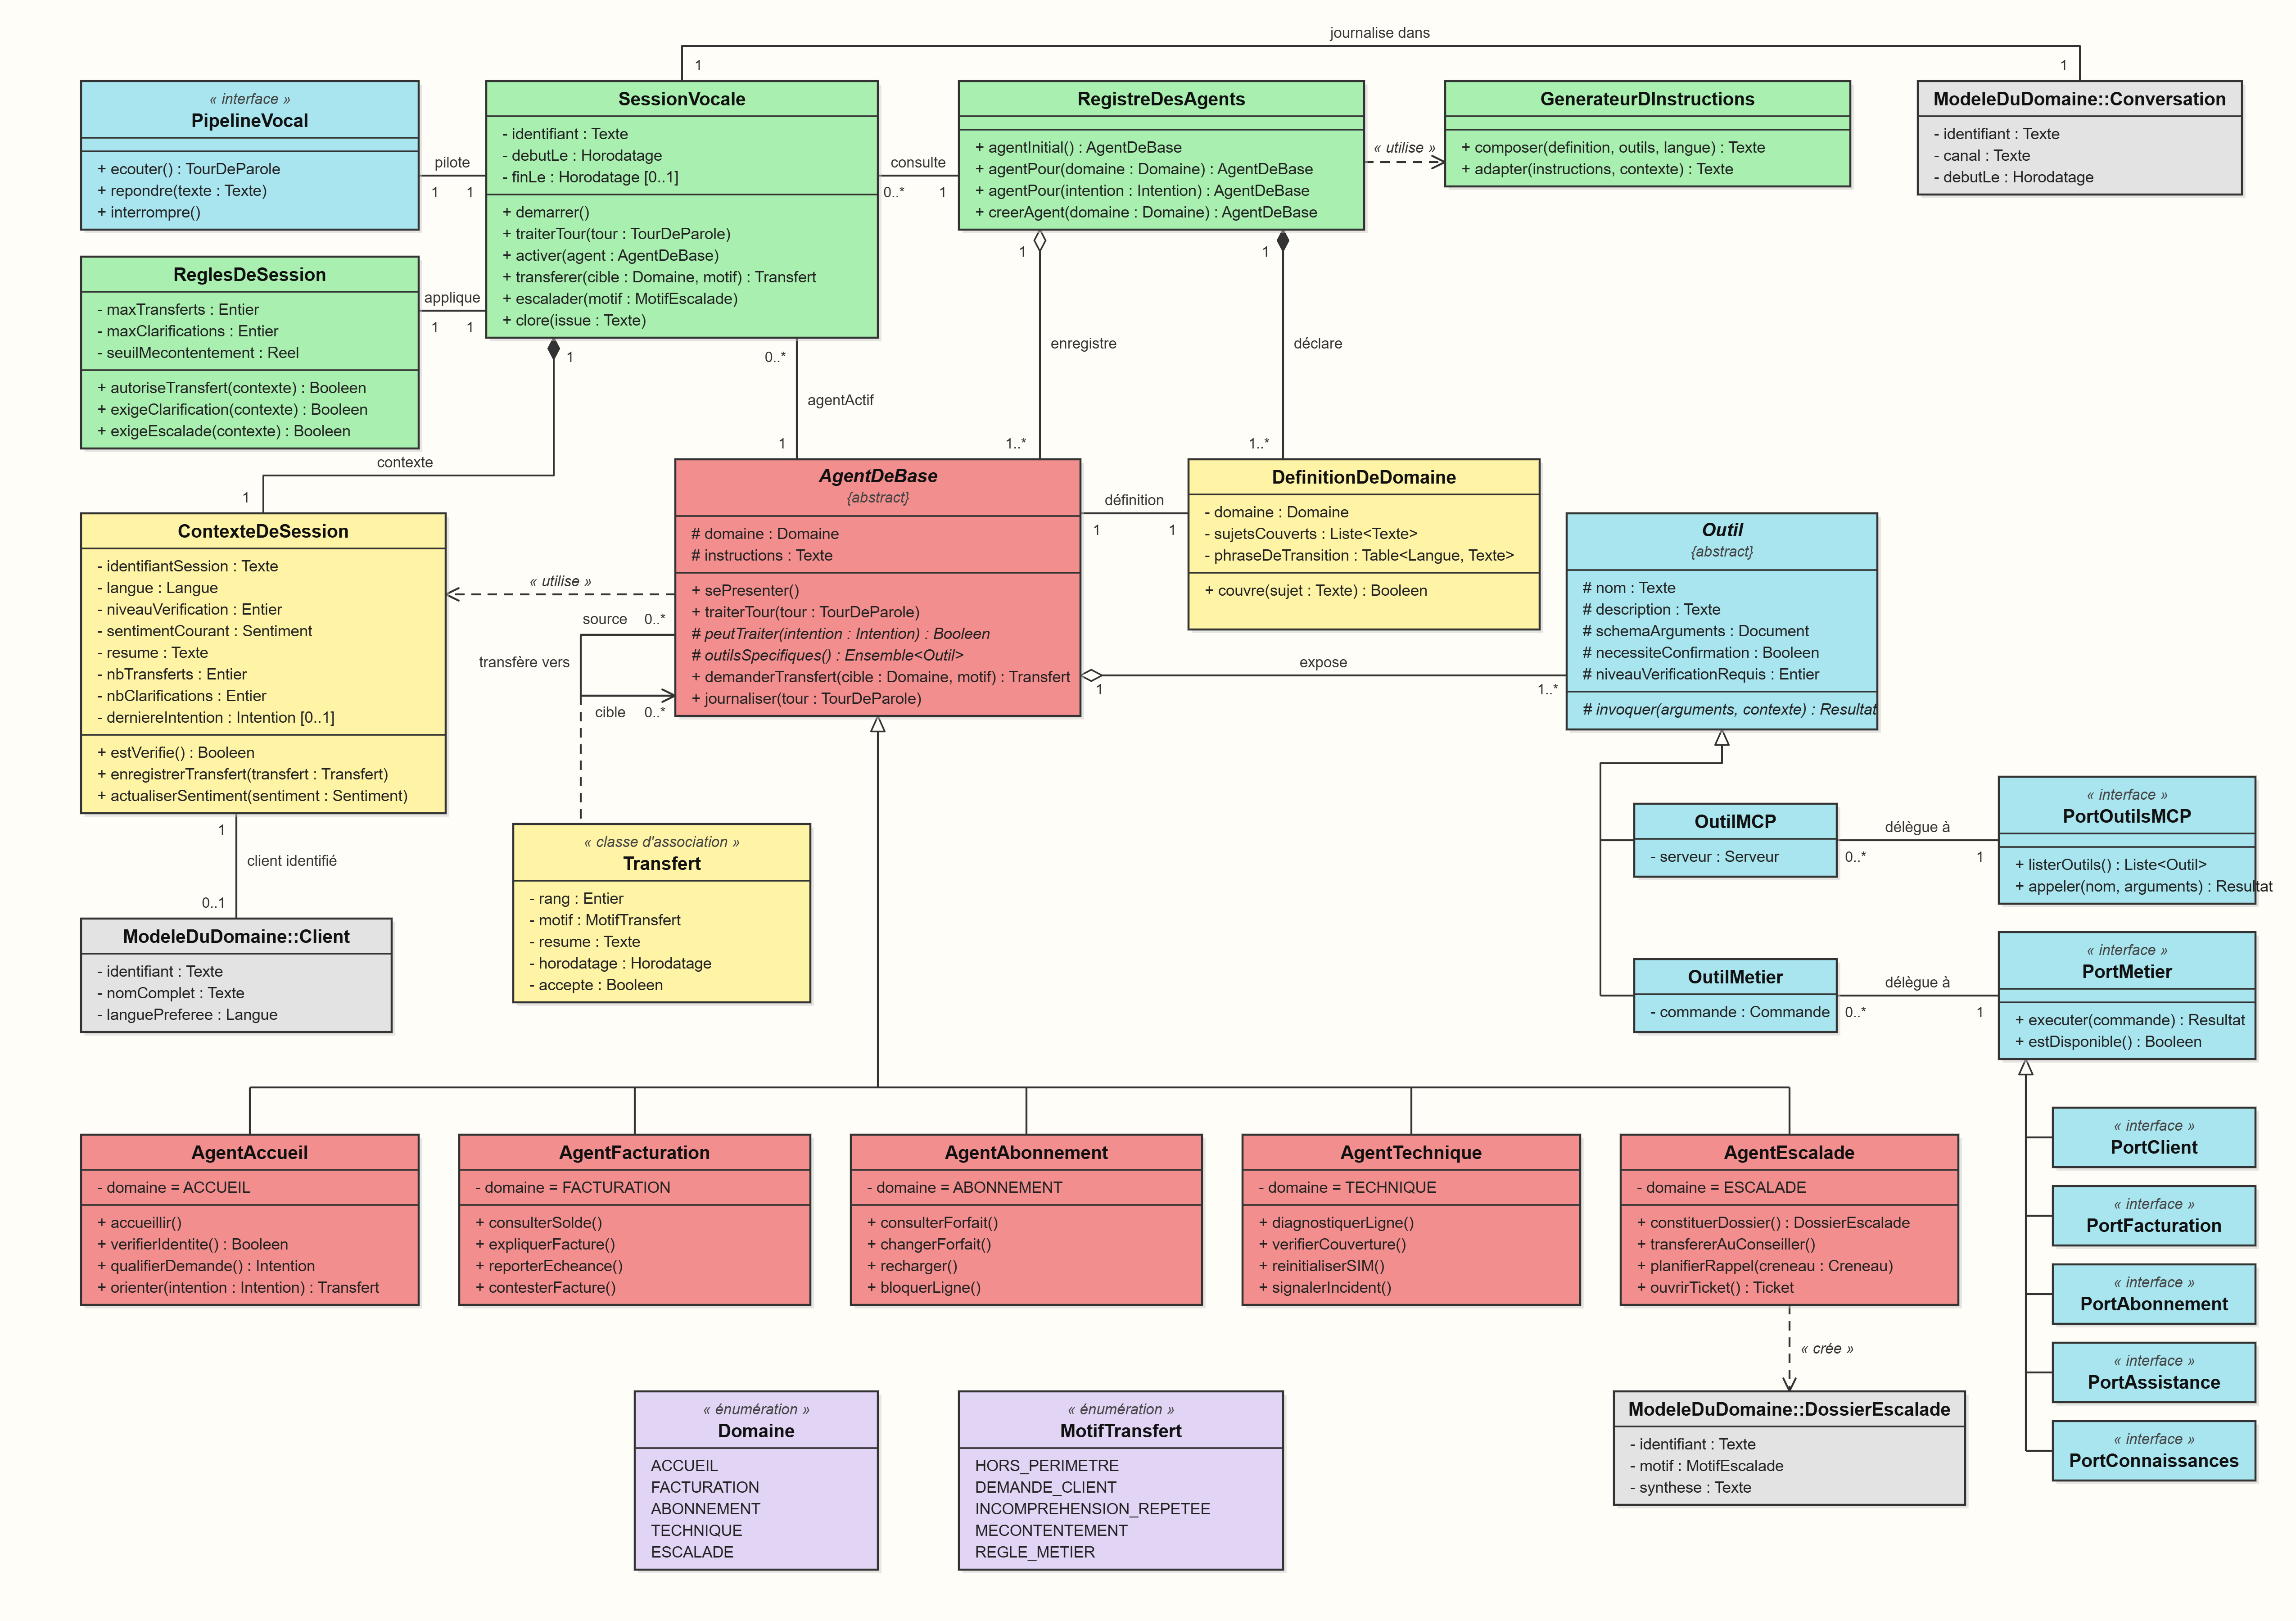
\includegraphics[width=\linewidth, height=0.82\textheight, keepaspectratio]{figures/fig-classes-agents.png}}
    \vspace{0.2cm}
    \caption{Diagramme de classes de la couche agents}
    \label{fig:classes-agents}
\end{figure}

\subsubsection{Moteur de décision déterministe}

Le moteur de politique ne juge pas une action directement. Il invoque d'abord un outil de la couche agents, qui construit le contexte de décision — action, arguments, domaine, client, niveau de vérification, sentiment courant, nombre de clarifications et canal. Il évalue ensuite ce contexte contre les règles de politique qu'il agrège, dans l'ordre de leur rang, en s'appuyant sur un calculateur de confiance.

Le contrat d'une règle est porté par l'interface \emph{RegleDePolitique}. Chaque règle expose son identifiant, son rang, la condition qui détermine si elle s'applique au contexte, puis l'évaluation elle-même. Celle-ci produit un objet valeur \emph{ResultatDeRegle} — verdict, justification, règle — ou ne se prononce pas, ce que traduit la multiplicité 0..1. Cette organisation reprend le patron de chaîne de responsabilité \cite{gamma} appliqué aux politiques : le moteur parcourt les règles dans l'ordre de leur rang et chacune s'applique ou s'abstient. Cinq règles concrètes réalisent cette interface, et leur ordre n'est pas arbitraire. \emph{RegleEscaladeObligatoire} porte le rang 1 et couvre l'abus, la menace, la fraude et le caractère juridique. Vient ensuite \emph{RegleVerificationIdentite}, appliquée aux actions sensibles. Les trois règles métier suivantes portent sur la facturation — plafond, échéance, litige —, l'abonnement — forfait, recharge, blocage — et le technique — carte SIM, réseau, incident.

Le moteur consolide les résultats recueillis et la confiance calculée en un \emph{VerdictDePolitique}. Cette classe porte la valeur rendue — autorisé, confirmation requise, refusé ou escalade —, le niveau de confiance, la justification, la règle décisive lorsqu'elle existe, la liste des facteurs de risque et l'horodatage. Elle expose les méthodes \emph{estAutorise()} et \emph{exigeConfirmation()}. Les facteurs de risque sont fermés par une énumération : identité non vérifiée, données manquantes, suspicion de fraude, mécontentement et clarifications répétées. Chaque verdict rendu est enfin consigné dans une entrée d'audit, qui porte l'événement, son contenu et son empreinte ; cette consignation rend le verdict reconstruit après coup, car elle permet de répondre non seulement à la question de savoir ce qui a été décidé, mais aussi à celle de savoir pourquoi.

La figure \ref{fig:classes-politique} présente ce moteur.

\begin{figure}[htbp]
    \centering
    \setlength{\fboxsep}{0pt}
    \setlength{\fboxrule}{1pt}
    \fbox{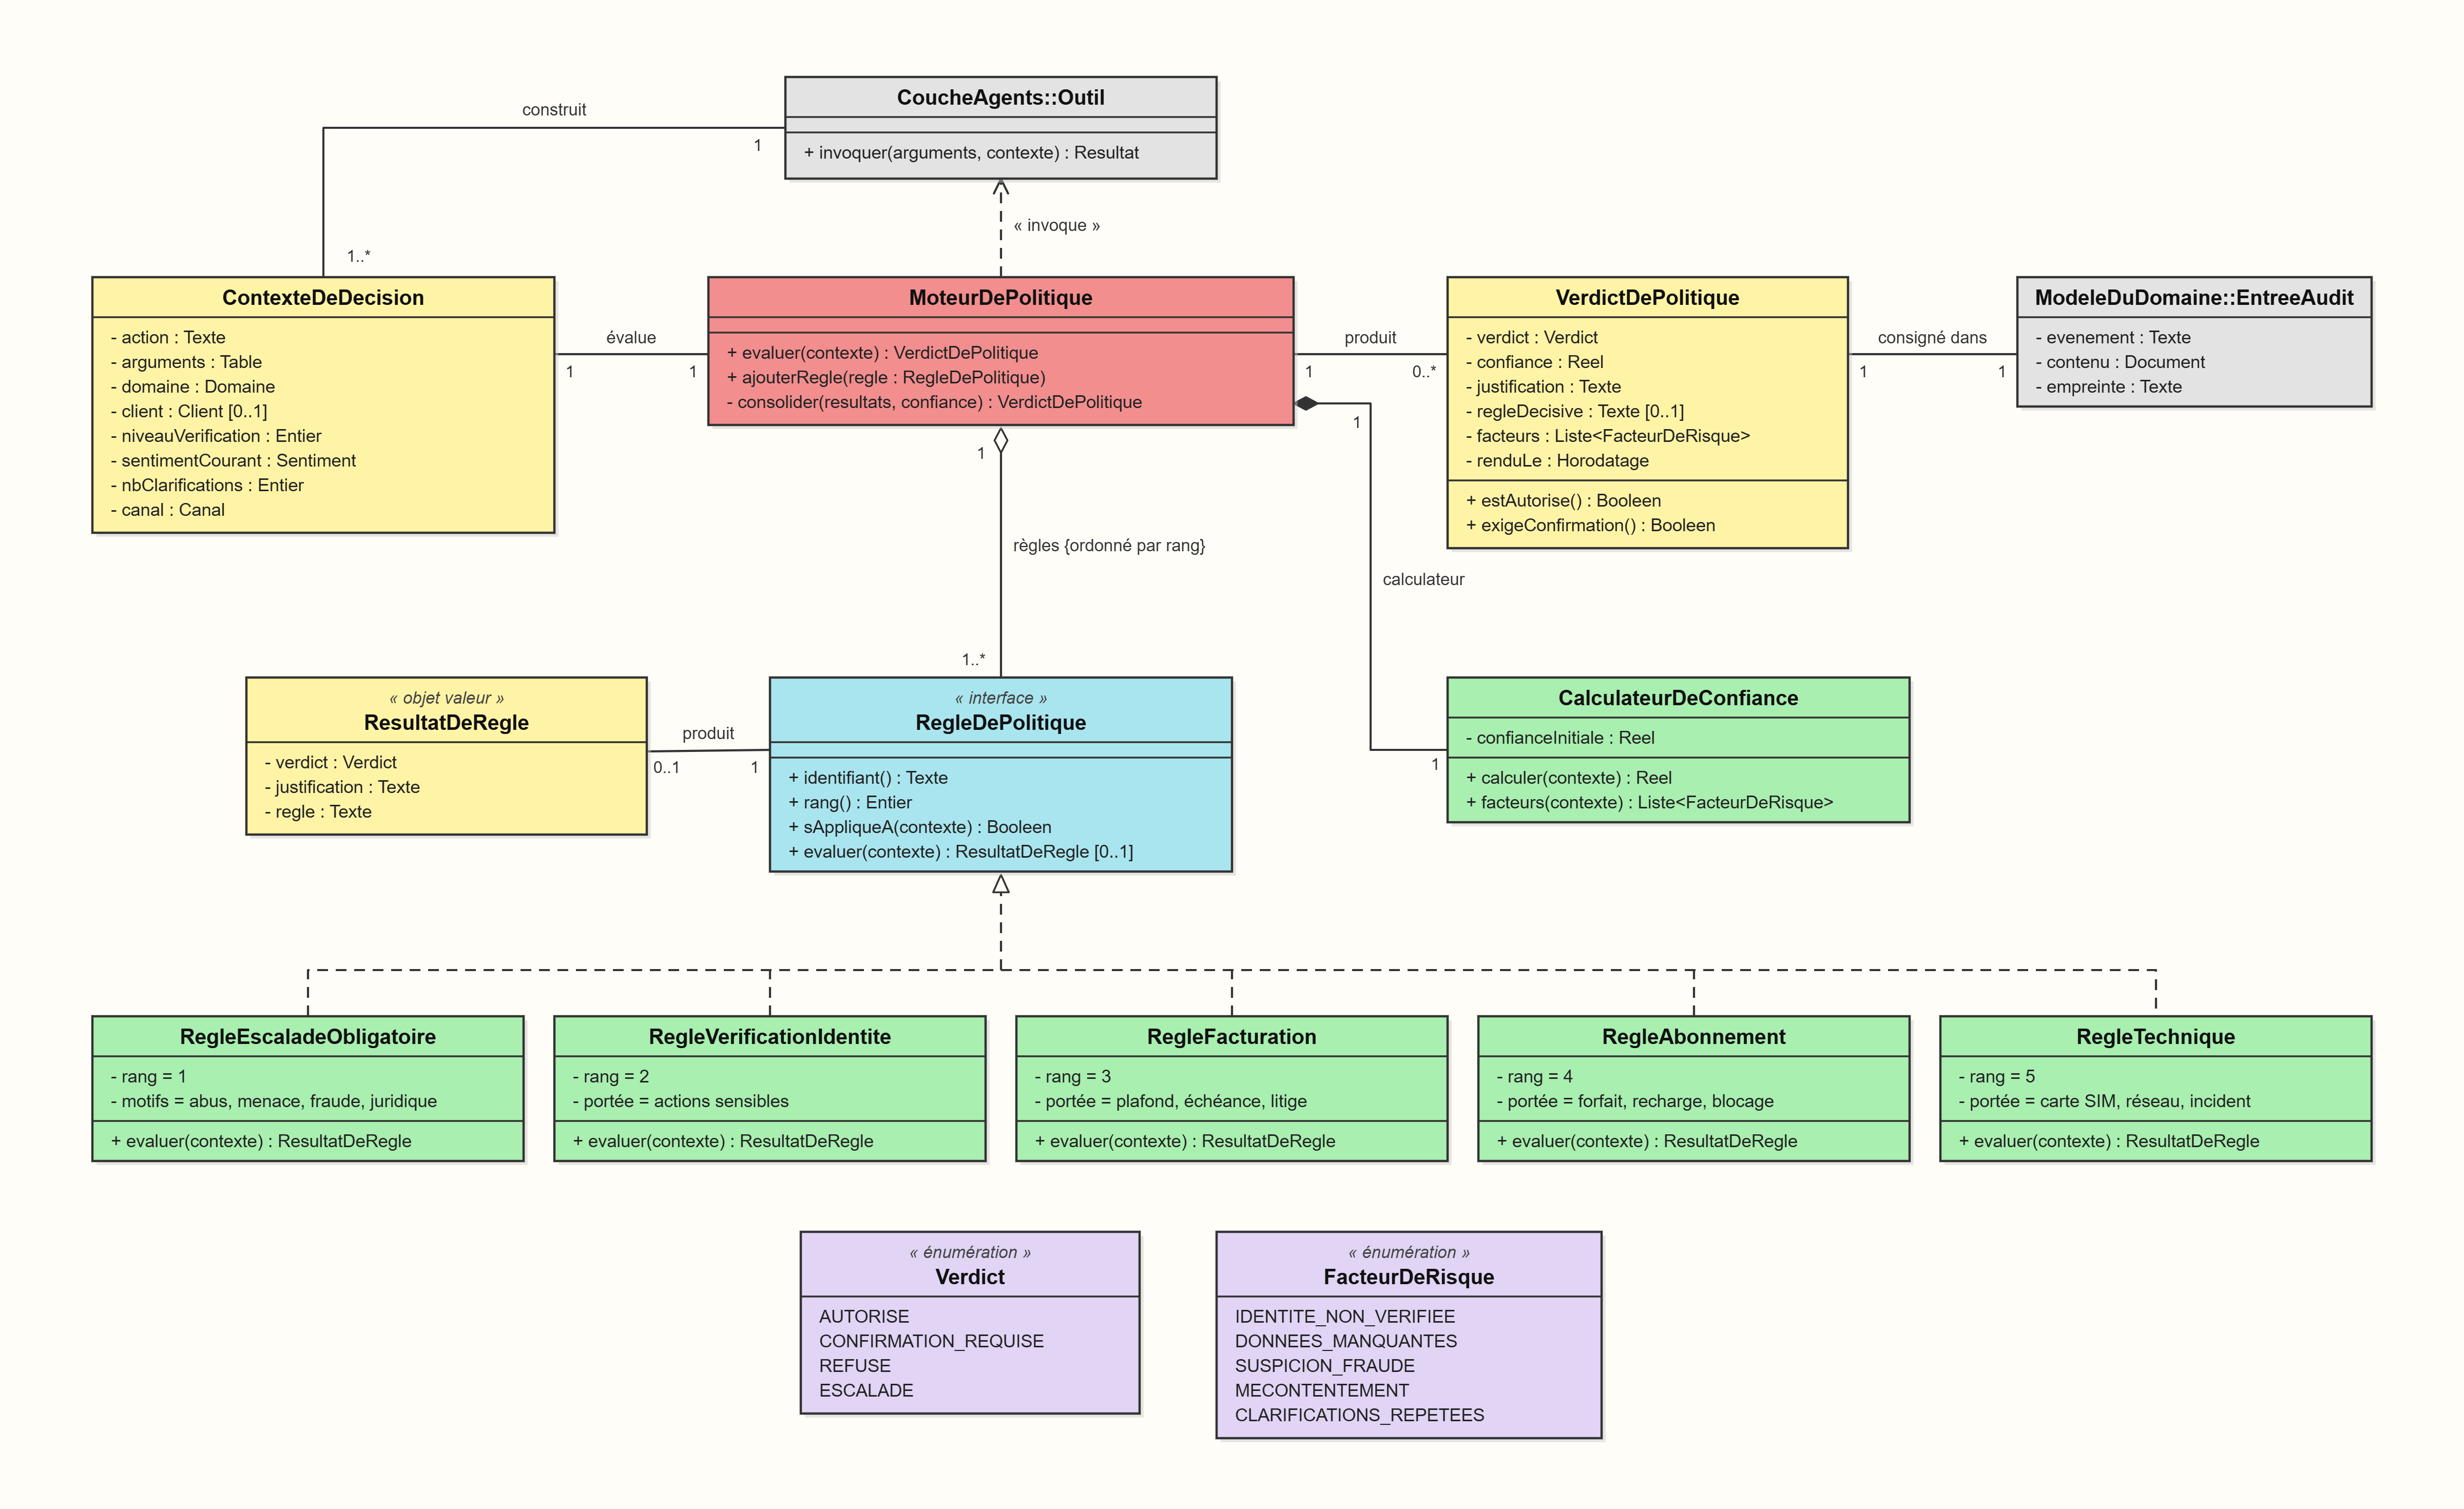
\includegraphics[width=\linewidth, height=0.82\textheight, keepaspectratio]{figures/fig-classes-politique.png}}
    \vspace{0.2cm}
    \caption{Diagramme de classes du moteur de politique}
    \label{fig:classes-politique}
\end{figure}


\section{Vue dynamique de l'application}

La vue statique a décrit les éléments du système. La vue dynamique décrit leur collaboration dans le temps. Nous retenons trois angles complémentaires : les diagrammes de séquence, qui montrent l'ordre exact des échanges entre composants, les diagrammes d'activités, qui montrent l'enchaînement algorithmique interne d'un traitement, et les diagrammes d'états transitions, qui montrent le cycle de vie des objets les plus significatifs.

\subsection{Diagrammes de séquence}

\subsubsection{Déroulement d'un tour de parole}

Le premier diagramme, présenté à la figure \ref{fig:seq-tour}, décrit le déroulement d'un tour de parole entre les huit participants de la chaîne vocale. Il représente le chemin le plus fréquemment emprunté du système, celui sur lequel pèse la contrainte de temps.

\begin{figure}[htbp]
    \centering
    \setlength{\fboxsep}{0pt}
    \setlength{\fboxrule}{1pt}
    \fbox{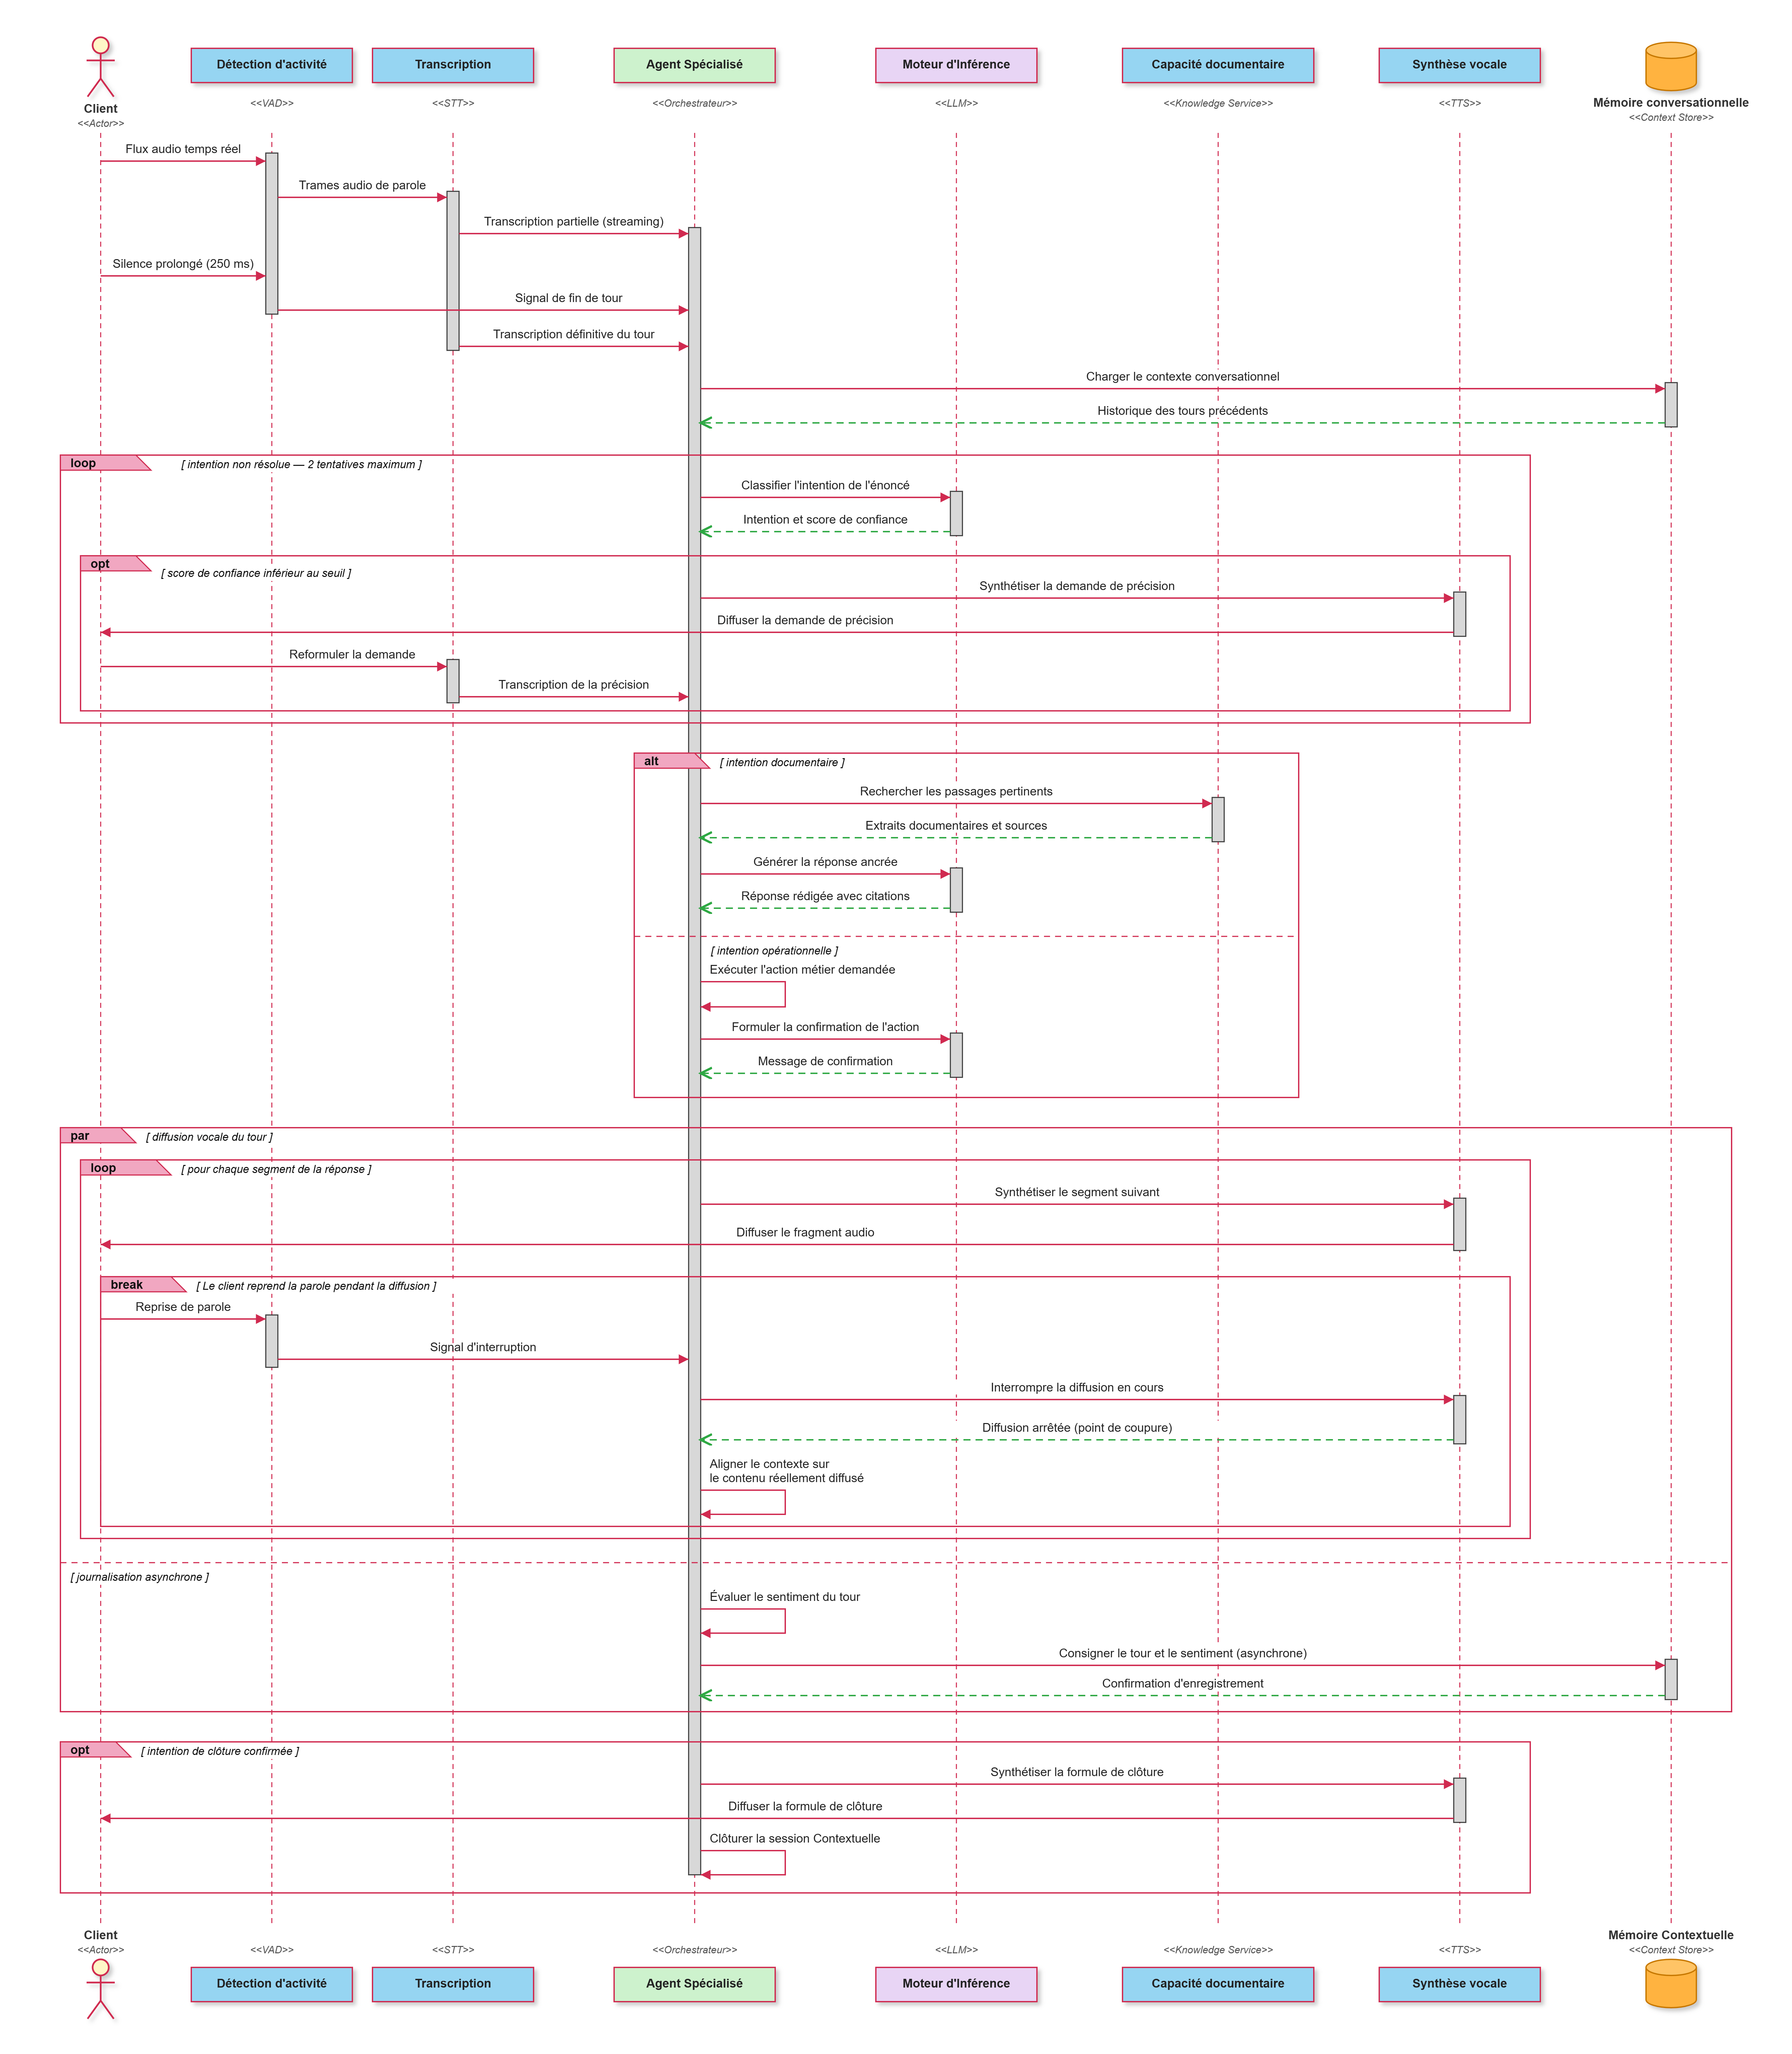
\includegraphics[width=\linewidth, height=0.88\textheight, keepaspectratio]{figures/fig-seq-tour.png}}
    \vspace{0.2cm}
    \caption{Diagramme de séquence du traitement d'un tour de parole}
    \label{fig:seq-tour}
\end{figure}

Le scénario commence par la capture du tour : la détection d'activité vocale transmet la transcription à l'agent, qui charge ensuite le contexte de la conversation. L'agent résout l'intention auprès du moteur d'inférence puis, selon le domaine, interroge la capacité documentaire ou exécute lui même l'action demandée.

La réponse est ensuite diffusée par fragments pendant que le tour et son sentiment sont journalisés. Si le client reprend la parole, la diffusion est interrompue et le contexte est réaligné ; si l'intention de clôture est confirmée, l'agent clôt la session.

\subsubsection{Déroulement d'une action sensible}

Le second diagramme, présenté à la figure \ref{fig:seq-sensible}, détaille la chaîne qui conduit de la demande du client à l'exécution effective d'une opération. Il représente le chemin le plus contraint du système.

\begin{figure}[htbp]
    \centering
    \setlength{\fboxsep}{0pt}
    \setlength{\fboxrule}{1pt}
    \fbox{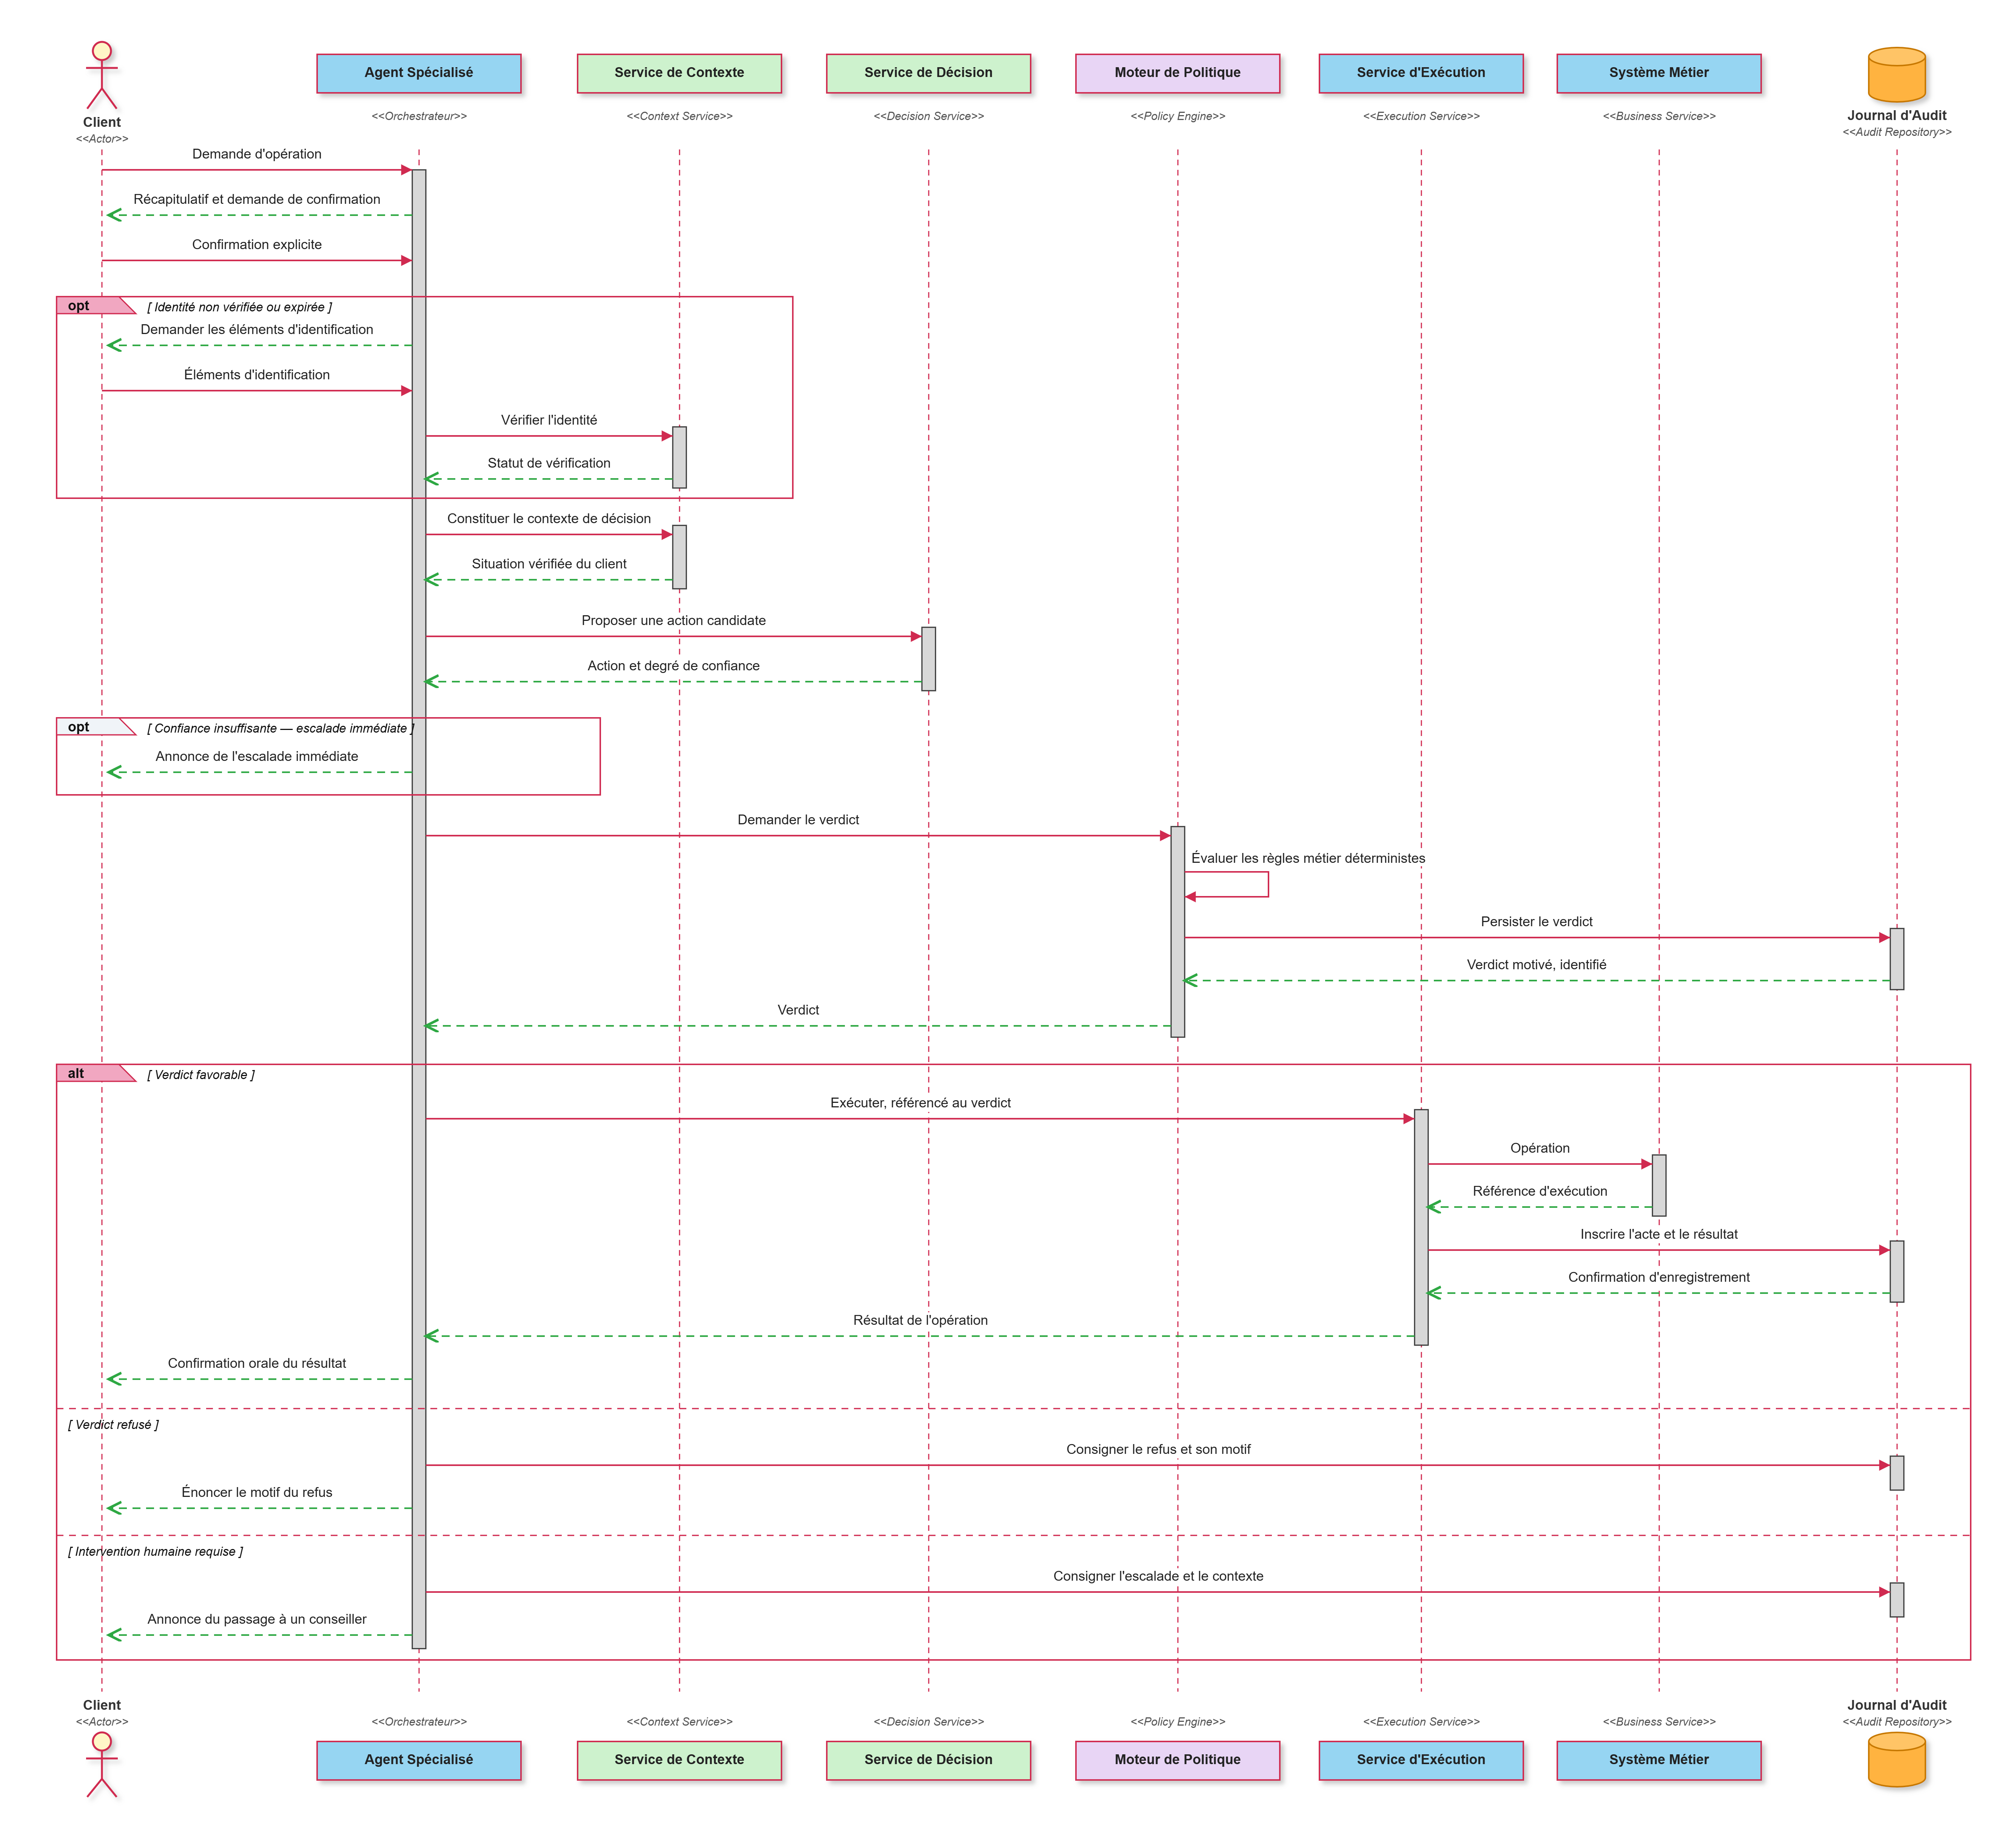
\includegraphics[width=\linewidth, height=0.88\textheight, keepaspectratio]{figures/fig-seq-sensible.png}}
    \vspace{0.2cm}
    \caption{Diagramme de séquence d'une action sensible}
    \label{fig:seq-sensible}
\end{figure}

L'agent confirme la demande puis vérifie l'identité du client si nécessaire. Le contexte de décision est ensuite constitué et le service de décision propose une action avec son degré de confiance ; une confiance insuffisante déclenche une escalade immédiate.

Le moteur de politique évalue ensuite l'action et persiste son verdict. Selon le résultat, l'opération est exécutée, refusée ou transmise à un conseiller ; chaque issue est inscrite dans le journal d'audit.


\subsection{Diagrammes d'activités}

\subsubsection{Ingestion documentaire}

Le diagramme de la figure \ref{fig:act-ingestion} décrit le traitement appliqué à un document versé dans la base documentaire. Ce traitement se déroule hors ligne, ce qui autorise un soin qui serait impossible pendant une conversation.

Le document est d'abord extrait de son format d'origine et converti en texte. Ses métadonnées sont ensuite déterminées, la langue étant déduite du contenu lorsqu'elle n'est pas déclarée. Le texte est alors segmenté en fragments de taille bornée, avec un recouvrement entre fragments consécutifs. La segmentation respecte les paragraphes plutôt que de découper à taille fixe, afin qu'un fragment demeure une unité de sens et non une tranche arbitraire ; seuls les paragraphes excédant la taille maximale sont scindés. Chaque fragment est ensuite encodé sous deux représentations complémentaires, l'une portant le sens et l'autre les termes exacts. L'ensemble est écrit en une seule transaction, accompagné d'un travail d'ingestion traçable et d'un événement de synchronisation. Un processus distinct consomme ces événements et met l'index à jour.

Deux décisions figurent explicitement dans ce diagramme. La première est le contrôle d'empreinte : un document dont le contenu est inchangé ne produit aucun travail, tandis qu'un contenu modifié engendre une nouvelle version et désactive la précédente. La seconde est le passage par une file d'événements durable plutôt qu'une écriture directe dans l'index. Si l'index est indisponible au moment de l'ingestion, l'événement demeure et sera traité ensuite, sans que la référence et l'index divergent durablement.

\figureTikz{Diagramme d'activités de l'ingestion documentaire}{act-ingestion}{fig-act-ingestion}

\subsubsection{Recherche documentaire}

Le diagramme de la figure \ref{fig:act-recherche} décrit le traitement d'une question, qui s'exécute cette fois sous contrainte de temps. Sa particularité tient à sa structure en filtres successifs, chacun pouvant conclure à l'absence de réponse.

La question est encodée puis soumise à une première sélection fondée sur la proximité de sens, avec un seuil minimal. Si aucun passage ne franchit ce seuil, le traitement s'arrête immédiatement sur un résultat vide. Les passages retenus sont ensuite confrontés à une seconde sélection fondée sur les termes exacts, qui écarte les passages dont le vocabulaire n'a rien de commun avec la question. Les deux classements sont alors fusionnés selon une méthode qui combine les rangs plutôt que les scores, ce qui évite d'avoir à ramener deux échelles de mesure hétérogènes à une échelle commune. Un dernier filtre évalue conjointement la question et chaque passage survivant, et n'en conserve que ceux dont la pertinence est confirmée.

Ce dernier filtre ne s'applique qu'au petit nombre de candidats ayant franchi les étapes précédentes. Cette restriction est ce qui rend son coût acceptable dans une chaîne temps réel, et le chapitre suivant en donne la mesure.

Le point essentiel de ce diagramme est la présence de trois sorties possibles vers un résultat vide. Ce n'est pas une faiblesse du traitement, mais sa propriété recherchée : le système préfère déclarer qu'il ne sait pas plutôt que remettre à l'agent des passages faiblement pertinents, sur lesquels il fonderait une réponse plausible mais infondée.

\figureTikz{Diagramme d'activités de la recherche documentaire}{act-recherche}{fig-act-recherche}

\subsection{Diagrammes d'états transitions}

\subsubsection{Cycle de vie d'une conversation}

Le diagramme de la figure \ref{fig:etats-conversation} décrit les états successifs d'une conversation. Il fait apparaître que la conversation possède deux issues terminales et non une seule : la résolution autonome et le passage à un conseiller. Les traiter symétriquement dans le modèle traduit la position adoptée au premier chapitre, selon laquelle l'escalade constitue un résultat normal du système et non une défaillance.

Un état mérite d'être signalé, celui de vérification d'identité. Il n'est atteint que lorsqu'une opération sensible est envisagée, il est borné en nombre de tentatives et dans le temps, et il possède sa propre sortie en échec. Cette délimitation stricte évite qu'une conversation ne s'enlise dans une boucle de vérification.

\figureTikz{Diagramme d'états transitions d'une conversation}{etats-conversation}{fig-etats-conversation}

\subsubsection{Cycle de vie d'un ticket}

Le diagramme de la figure \ref{fig:etats-ticket} décrit les états d'un ticket. Le vocabulaire d'états retenu est celui du système de référence de l'organisation, et non un vocabulaire propre à la plateforme : cinq états, de l'ouverture à la clôture, avec un état d'attente distinct de l'état de traitement en cours.

Ce choix de reprendre le vocabulaire du système de référence évite une correspondance approximative entre deux jeux d'états, source classique d'incohérences lorsque les deux systèmes évoluent séparément. La plateforme traduit les codes numériques du système de référence vers ces cinq états, et cette traduction est le seul point où les deux vocabulaires se rencontrent.

\figureTikz{Diagramme d'états transitions d'un ticket}{etats-ticket}{fig-etats-ticket}

\section{Conception du système agentique}

Les deux sections précédentes ont décrit la structure et la dynamique générales du système. Celle ci traite de sa couche la plus spécifique, celle qui conduit la conversation et décide de ce qu'il convient de faire. Nous en présentons le principe, la décomposition, la construction du contexte, la gestion de la mémoire, puis les mécanismes qui encadrent le comportement.

\subsection{Principe et pipeline de raisonnement}

Un agent, au sens retenu ici, n'est pas un modèle de langue auquel on adresse une question. C'est un composant qui reçoit une demande, dispose d'un ensemble borné de capacités, se voit imposer un ensemble de contraintes, et produit soit une réponse, soit l'appel d'une capacité, soit une transmission à un autre agent.

Son fonctionnement suit un enchaînement en quatre temps. L'agent interprète d'abord la demande à la lumière de son contexte. Il détermine ensuite ce qu'il convient de faire, ce qui peut consister à répondre directement, à solliciter une capacité, ou à passer la main. Cette intention est alors soumise aux contraintes applicables, qui peuvent la valider, la refuser ou imposer une intervention humaine. L'action n'est réalisée qu'à l'issue de cette validation, et son résultat est restitué au client.

La distinction entre le deuxième et le troisième temps est la clé de la conception. Le modèle de langue intervient au deuxième temps, où sa capacité d'interprétation est irremplaçable. Il n'intervient pas au troisième, où c'est un mécanisme déterministe qui statue. Le modèle propose, il ne dispose pas. La figure \ref{fig:pipeline-agent} présente cet enchaînement.

\figureTikz{Pipeline de raisonnement d'un agent}{pipeline-agent}{fig-pipeline-agent}

\subsection{Décomposition en agents spécialisés}

\subsubsection{Motivation}

Un agent unique chargé de l'ensemble des domaines pose trois difficultés. Ses instructions deviennent longues, et une instruction longue est moins bien suivie qu'une instruction courte. Ses capacités deviennent nombreuses, et un ensemble de capacités étendu augmente la probabilité d'un appel inapproprié. Enfin, toute évolution d'un domaine impose de reconsidérer l'ensemble, puisque rien n'est isolé.

Nous avons donc réparti la charge entre cinq agents. Un agent d'accueil ouvre la conversation et détermine la nature de la demande. Trois agents spécialisés couvrent chacun un domaine métier : la facturation, l'abonnement et le technique. Un agent d'escalade traite les situations qui débordent des trois domaines métier et pilote les cas d'escalade. Chacun ne porte que les instructions et les capacités de son périmètre.

\subsubsection{Déclaration unique des domaines}

Une décomposition de ce type comporte un risque connu : la désynchronisation entre ce qu'une instruction annonce et ce que l'outillage permet réellement. Un agent à qui l'on demande de transmettre une demande vers un domaine dont la capacité de transfert n'est pas déclarée se trouve dans une situation sans issue, dont il sortira par un comportement imprévisible.

La conception écarte ce risque en déclarant chaque domaine une seule fois, dans une table qui constitue la référence unique. Cette table associe à chaque domaine les sujets qu'il couvre, la capacité de transfert correspondante et la phrase de transition énoncée au client dans chacune des langues prises en charge. Les instructions des agents comme leur outillage sont dérivés de cette même table. Il devient donc structurellement impossible qu'un domaine soit nommé dans une consigne sans que la capacité associée existe.

Le tableau \ref{tab:domaines} présente cette déclaration.

\begin{table}[H]
\centering
\renewcommand{\arraystretch}{1.25}
\begin{tabular}{|p{3.0cm}|p{6.2cm}|p{5.3cm}|}
\hline
\textbf{Domaine} & \textbf{Sujets couverts} & \textbf{Traitement de la transition} \\
\hline
Facturation & Solde, facture, règlement, report d'échéance & Phrase de transition déterministe, énoncée dans la langue de l'échange \\
\hline
Abonnement & Forfait, recharge, itinérance, ligne téléphonique & Idem \\
\hline
Technique & Carte SIM, réseau, connectivité & Idem \\
\hline
\end{tabular}
\caption{Déclaration unique des domaines de spécialité}
\label{tab:domaines}
\end{table}

Le caractère déterministe de la phrase de transition mérite une justification. Il serait possible de laisser le modèle formuler lui même l'annonce du transfert. Nous ne l'avons pas fait, parce que cette phrase est un engagement pris envers le client : elle annonce un événement qui va se produire. Une formulation générée pourrait annoncer un transfert vers un service qui n'existe pas, ou promettre un délai. Une phrase fixe ne le peut pas.

\subsubsection{Passage de relais entre agents}

Lorsqu'un agent transmet la conversation à un autre, le contexte déjà constitué est conservé : le client n'a pas à se réidentifier ni à reformuler sa demande. Ce comportement est la traduction directe du besoin exprimé au chapitre précédent, où la perte de contexte lors des transferts avait été identifiée comme l'une des faiblesses majeures du dispositif existant.

Le passage de relais est par ailleurs encadré par un garde fou contre les boucles. Le nombre de transferts et le rang du tour de parole auquel le dernier a eu lieu sont suivis, de sorte que deux agents ne puissent pas se renvoyer indéfiniment une demande qu'aucun des deux ne reconnaît comme sienne. Au delà d'un certain nombre de passages, la demande est traitée comme débordant des domaines couverts. Cette borne est portée par le contexte de session et contrôlée par les règles de session, tandis que chaque passage est consigné par la classe d'association \emph{Transfert}.

La figure \ref{fig:orchestration} présente l'organisation des agents et les transitions possibles entre eux.

\figureTikz{Orchestration des agents et transitions}{orchestration}{fig-orchestration}

\subsection{Construction du contexte}

\subsubsection{Un contexte assemblé et non accumulé}

Le contexte fourni à un agent n'est pas un historique qui grossit à chaque tour. C'est un assemblage, reconstitué à partir de sources distinctes, dont chacune n'est sollicitée que lorsqu'elle est utile.

Cette distinction a une portée pratique directe. Tout élément placé dans le contexte consomme une part de la fenêtre disponible et une part du temps de traitement. Un contexte qui accumule tout devient à la fois plus coûteux et moins efficace, car l'information pertinente s'y dilue. Le tableau \ref{tab:contexte} récapitule les sources du contexte et leur condition de sollicitation.

\begin{table}[H]
\centering
\renewcommand{\arraystretch}{1.2}
\begin{tabular}{|p{4.0cm}|p{5.0cm}|p{5.5cm}|}
\hline
\textbf{Source} & \textbf{Contenu} & \textbf{Condition de sollicitation} \\
\hline
Identité de session & Identifiant de session, langue courante, rang du tour & Systématique \\
\hline
Profil client & Nom, numéro de ligne, type d'abonnement, statut particulier & À l'ouverture de la conversation \\
\hline
Situation de facturation & Montants dus, factures ouvertes & Sur demande relevant du domaine facturation \\
\hline
Historique des demandes & Tickets et réclamations en cours & Sur demande le justifiant \\
\hline
Mémoire d'appels antérieurs & Faits structurés issus des échanges précédents & À l'ouverture, si le client a un historique \\
\hline
État de vérification & Identité vérifiée, niveau, horodatage, échéance & Avant toute opération sensible \\
\hline
Sentiment courant & Score cumulé et nombre de tours négatifs consécutifs & Systématique, en arrière plan \\
\hline
Connaissance documentaire & Passages pertinents et leur source & Sur question documentaire uniquement \\
\hline
Outils disponibles & Ensemble des outils exposés par l'agent actif & Déterminé par l'agent actif \\
\hline
\end{tabular}
\caption{Sources du contexte et conditions de sollicitation}
\label{tab:contexte}
\end{table}

La figure \ref{fig:contexte} illustre cet assemblage.

\figureTikz{Assemblage du contexte d'un agent}{contexte}{fig-contexte}

\subsubsection{Mémoire courte et mémoire longue}

Deux mémoires coexistent, de nature différente.

La mémoire courte est celle de la conversation en cours. Elle conserve les tours de parole, l'état de vérification, les compteurs de clarification et de transfert, l'évolution du sentiment et les identités des opérations engagées. Elle disparaît avec la session. C'est elle qui rend le passage de relais transparent et offre à l'agent qui reprend la conversation le même fil, sans obliger le client à se répéter.

La mémoire longue traverse les appels. Elle permet qu'un client rappelant au sujet d'un incident déjà signalé n'ait pas à tout réexpliquer. Elle est présentée à l'agent sous forme de faits structurés, et non d'une synthèse rédigée. Une synthèse est une affirmation sur ce qui a été dit, produite par le même type de modèle qui la relira ensuite comme un fait acquis ; si elle est subtilement fausse, elle le reste à chaque appel. Les faits structurés, au contraire, sont re-dérivés à chaque lecture à partir des échanges conservés : ils bornent le coût sans figer une interprétation susceptible de devenir une source d'erreur persistante.

Trois règles de conception encadrent cette mémoire longue, et chacune répond à un défaut identifié.

\begin{itemize}
  \item \textbf{Ne jamais accueillir le client par ce dont on se souvient.} Un assistant qui ouvre l'échange en énumérant les appels précédents produit une impression de surveillance, et présume par ailleurs du motif de l'appel, qui peut être tout autre. La mémoire est un contexte mobilisable lorsqu'il devient pertinent, non une entrée en matière.
  \item \textbf{Ne jamais présenter un élément de mémoire comme un fait actuel.} Un élément consigné comme ouvert l'était au moment où il a été recueilli. Affirmer au client qu'il l'est encore constitue une assertion sur le présent, qui exige une relecture de l'état courant avant d'être formulée.
  \item \textbf{Ne rien dire lorsqu'il n'y a rien.} Un premier appel et un client ayant désactivé la mémorisation produisent l'un comme l'autre une mémoire vide, qui n'ajoute ni contenu ni comportement.
\end{itemize}

Lorsque le client demande l'effacement des informations mémorisées, la demande est enregistrée comme un état de remise à zéro : la mémoire repart vide à l'appel suivant, tandis que l'historique de la conversation et la chaîne d'audit demeurent intacts.

Ces règles illustrent une orientation générale de la conception : une capacité n'est utile que si ses conditions d'usage sont définies avec autant de soin que la capacité elle même.

\subsection{Garde fous et comportement déterministe}

\subsubsection{Nature des garde fous}

Les garde fous encadrent ce que le système peut décider et ce qu'il peut dire. Ils s'appliquent à deux moments distincts, ce qui constitue une propriété importante de la conception.

Le premier moment précède l'action. Toute opération sensible est soumise au moteur de politique décrit plus haut, qui rend un verdict à quatre valeurs accompagné de la règle décisive, du niveau de confiance et d'une justification. Ce contrôle n'est pas contournable, puisque le chemin qui mène à l'exécution passe par lui.

Le second moment précède la parole. Une réponse sur le point d'être énoncée peut être contrôlée avant son émission, notamment au regard de la divulgation de données personnelles, de la formulation d'engagements ou de la mention de montants. Une plateforme qui contrôlerait ses actions sans contrôler ses paroles laisserait ouverte une voie de préjudice pourtant réelle.

\subsubsection{Le sentiment comme signal de décision}

Le sentiment exprimé par le client constitue un signal supplémentaire, distinct des règles métier. Sa conception a évolué au cours du projet, et l'évolution est instructive.

Le modèle initial comptait les tours négatifs consécutifs et déclenchait une escalade au troisième. Il s'est révélé à la fois trop sensible et trop indulgent. Trop sensible, parce qu'un seul mot vif portait le score au maximum et y maintenait la conversation entière. Trop indulgent, parce que tout tour non négatif remettait le compteur à zéro, de sorte qu'un client mécontent de manière constante mais courtoise n'était jamais détecté.

Le modèle retenu procède par accumulation. Un tour négatif fait progresser un score, un tour positif le fait décroître, et une expression d'agressivité pèse plus lourd qu'un simple mécontentement. Le seuil est atteint par trois tours négatifs, ce qui préserve le comportement de référence, mais une seule phrase vive ne suffit plus, et un apaisement réel est effectivement pris en compte.

Le tableau \ref{tab:sentiment} illustre le comportement obtenu.

\begin{table}[H]
\centering
\renewcommand{\arraystretch}{1.25}
\begin{tabular}{|p{6.5cm}|p{3.2cm}|p{4.5cm}|}
\hline
\textbf{Séquence de tours} & \textbf{Score atteint} & \textbf{Conséquence} \\
\hline
Trois tours négatifs & 0,66 & Seuil franchi, escalade proposée \\
\hline
Deux tours négatifs & 0,44 & Sous le seuil, pas d'escalade \\
\hline
Négatif, positif, négatif & 0,26 & Sous le seuil, l'apaisement est pris en compte \\
\hline
Expression d'agressivité & 0,55 & Proche du seuil, traitement dédié \\
\hline
\end{tabular}
\caption{Comportement du modèle d'accumulation du mécontentement}
\label{tab:sentiment}
\end{table}

Il importe de souligner que ce signal n'autorise ni ne refuse rien par lui même. Il alimente la décision d'escalade, laquelle demeure soumise aux mêmes règles que les autres.

\subsubsection{Déterminisme là où il compte}

La conception rend délibérément déterministes plusieurs comportements qu'il aurait été plus simple de confier au modèle de langue. Le tableau \ref{tab:determinisme} recense ces choix et leur motif.

\begin{table}[H]
\centering
\renewcommand{\arraystretch}{1.25}
\begin{tabular}{|p{5.2cm}|p{9.3cm}|}
\hline
\textbf{Comportement rendu déterministe} & \textbf{Motif} \\
\hline
Verdict sur une action sensible & Une décision engageant un compte client doit être reproductible et justifiable par une règle identifiée. \\
\hline
Phrase de transition entre agents & Elle annonce un événement qui va se produire ; une formulation libre pourrait promettre autre chose. \\
\hline
Énoncés de la vérification d'identité & Le nombre de tentatives et les formulations sont bornés, ce qui évite l'enlisement et les reformulations hasardeuses. \\
\hline
Dates et heures de rappel & Un horaire inventé est pire que l'absence de rendez vous ; les créneaux proviennent des disponibilités réelles et sont mis en forme, non générés. \\
\hline
Identité d'une opération & Elle garantit l'exécution unique et ne peut dépendre d'une interprétation. \\
\hline
Abstention documentaire & En l'absence de passage pertinent, la réponse est fixée et non reformulée. \\
\hline
\end{tabular}
\caption{Comportements rendus déterministes et motifs associés}
\label{tab:determinisme}
\end{table}

\subsection{Du prompt au harnais}

La conception de cette couche s'inscrit dans une progression que le projet a parcourue et qu'il est utile d'expliciter, car elle éclaire l'essentiel des choix précédents.

La première approche consiste à soigner les instructions données au modèle. Elle produit rapidement des résultats et atteint tout aussi rapidement ses limites : une instruction longue est appliquée de manière inégale, et rien ne garantit qu'elle le soit du tout.

La deuxième approche déplace l'attention vers ce que le modèle reçoit. Elle consiste à choisir les informations mises à sa disposition, à les assembler au moment opportun et à gérer leur durée de vie. C'est ce que décrit la sous section consacrée à la construction du contexte.

La troisième approche porte sur le système qui entoure le modèle : ce qui borne ses capacités, ce qui valide ses intentions, ce qui contrôle ses énoncés, ce qui enregistre ses décisions et ce qui reprend la main lorsqu'il échoue. C'est cette approche qui structure la plateforme.

La conclusion pratique de cette progression est qu'un appel unique à un modèle, aussi soigneusement formulé soit il, ne peut porter un système de cette nature. Ce n'est pas la qualité des instructions qui garantit le comportement, c'est l'architecture qui les entoure.

\section{Conception de la sécurité et du contrôle d'accès}

\subsection{Deux frontières distinctes}

La sécurité de la plateforme repose sur une distinction qu'il convient d'énoncer d'emblée, car la confondre constituerait une faille.

La première frontière contrôle l'accès à la plateforme : qui se connecte, et à quelles fonctions ce profil donne droit. La seconde contrôle l'exécution des opérations sensibles à l'intérieur de la plateforme : le fait qu'un client soit connecté à son espace ne suffit pas à autoriser une opération sur son compte lors d'une conversation vocale.

Ces deux frontières sont indépendantes. Une session ouverte franchit la première et ne dit rien de la seconde. La figure \ref{fig:securite} présente ce modèle.

\figureTikz{Modèle de sécurité de la plateforme}{securite}{fig-securite}

\subsection{Authentification et gestion de session}

L'authentification est centralisée et commune aux deux catégories d'utilisateurs, qui sont ensuite orientées vers des espaces distincts selon leur rôle. Les éléments d'authentification sont conservés sous forme dérivée au moyen d'une fonction de dérivation à coût mémoire élevé \cite{scrypt}, dont les paramètres sont enregistrés avec chaque empreinte, de manière à pouvoir être renforcés ultérieurement sans invalider les comptes existants ni imposer une migration.

Une session authentifiée n'est pas un jeton autoportant dont la validité s'apprécierait à sa seule lecture. Elle est revalidée auprès de son enregistrement à chaque requête. La conséquence pratique est qu'une déconnexion, une expiration ou une révocation de l'ensemble des sessions d'un utilisateur prennent effet immédiatement, et non à l'échéance du jeton.

\subsection{Autorisation fondée sur le rôle}

L'autorisation repose sur trois rôles internes, auxquels s'ajoute le rôle client. Le diagramme de cas d'utilisation général du chapitre précédent les réunit sous un acteur unique, l'utilisateur back-office, afin de ne pas surcharger la vue d'ensemble ; la matrice ci-dessous en précise la répartition réelle. L'administrateur gère les connaissances et les règles métier, le superviseur assume la supervision des interactions, et le conseiller prend en charge les demandes escaladées. Chaque rôle dispose des droits du niveau précédent, augmentés des siens. Le tableau \ref{tab:rbac} présente la matrice des droits.

\begin{table}[H]
\centering
\renewcommand{\arraystretch}{1.2}
\begin{tabular}{|p{5.1cm}|p{1.9cm}|p{2.2cm}|p{2.2cm}|p{2.2cm}|}
\hline
\textbf{Ressource} & \textbf{Client} & \textbf{Conseiller} & \textbf{Super\-viseur} & \textbf{Admini\-strateur} \\
\hline
Ses propres données et conversations & Oui & Non & Non & Non \\
\hline
Assistant conversationnel & Oui & Non & Non & Non \\
\hline
Données d'un autre client & Non & Non & Non & Non \\
\hline
Rappels et disponibilités & Non & Oui & Oui & Oui \\
\hline
Conversations et transcriptions & Non & Non & Oui & Oui \\
\hline
Décisions et verdicts & Non & Non & Oui & Oui \\
\hline
Indicateurs d'activité & Non & Non & Oui & Oui \\
\hline
Comptes et règles métier & Non & Non & Non & Oui \\
\hline
Base documentaire & Non & Non & Non & Oui \\
\hline
Registre d'audit et vérification & Non & Non & Non & Oui \\
\hline
\end{tabular}
\caption{Matrice des droits par rôle}
\label{tab:rbac}
\end{table}

Trois principes gouvernent l'application de cette matrice.

Le premier est que le rôle n'est jamais déclaré par l'appelant. Il est déterminé à partir de la session que le système a lui même émise. Une conception antérieure du projet lisait le rôle dans un en tête de requête, ce qui revenait à laisser le client déclarer ses propres droits. Ce mécanisme a été supprimé, et l'en tête correspondant est aujourd'hui ignoré.

Le deuxième est que le contrôle côté interface ne constitue pas une protection. Les fonctions serveur étant atteignables indépendamment de la page qui les appelle, une vérification effectuée à l'affichage serait contournable. Le contrôle est donc appliqué sur chaque fonction serveur, et la vérification côté interface ne sert qu'à éviter un aller retour voué à l'échec.

Le troisième est le refus par défaut. En l'absence d'information d'autorisation exploitable, la demande est rejetée. Un rôle par défaut avait initialement été défini au niveau de la configuration, ce qui rendait l'ensemble des points d'accès atteignables ; ce défaut a été supprimé au profit d'un comportement fermé.

\subsection{Isolation des données entre clients}

Un client ne doit atteindre que ses propres données. Cette exigence, qui paraît évidente, se traduit par une contrainte de conception précise : la vérification ne peut porter sur l'identifiant transmis dans la requête, puisque celui ci est sous le contrôle de l'appelant. Elle porte sur la correspondance entre la ressource demandée et l'identité établie par la session. Une demande formulée par un client au sujet d'un autre est refusée, non parce que l'interface ne l'a pas proposée, mais parce que le serveur constate la discordance.

\subsection{Vérification d'identité renforcée}

Les opérations sensibles engagées au cours d'une conversation exigent une vérification distincte, fondée sur un élément que seul le titulaire connaît. Cette vérification est bornée à plusieurs égards : le nombre de tentatives est limité, le nombre de réponses inexploitables l'est également, et l'ensemble est soumis à une échéance.

Trois délais sont par ailleurs ordonnés de manière stricte : celui de l'appel de vérification, celui de la procédure complète, et celui du contrôle qui l'englobe. Cet ordre garantit que chaque niveau expire avant celui qui le contient, de sorte qu'une défaillance soit signalée à son niveau réel plutôt qu'absorbée par le délai supérieur, où elle deviendrait indiscernable.

Le résultat de la vérification n'est pas un simple indicateur booléen. Il porte l'identifiant du client vérifié, le niveau atteint, l'horodatage et l'échéance. Une vérification est donc valable pour un client déterminé et pour une durée déterminée, ce qui interdit qu'une vérification obtenue dans un contexte serve dans un autre.

\subsection{Traçabilité}

Toute opération administrative ou sensible laisse une trace comportant l'identité de son auteur, son rôle, l'action réalisée, la ressource concernée, l'horodatage, le résultat et le verdict d'autorisation. Les données personnelles y sont masquées partout où leur valeur exacte n'est pas nécessaire.

Ces traces sont organisées en chaîne : chaque enregistrement intègre l'empreinte du précédent dans le calcul de la sienne, au moyen d'une fonction de hachage cryptographique normalisée \cite{sha}. La modification d'un enregistrement ancien invalide donc toutes les empreintes postérieures, ce qui rend l'altération détectable par un simple recalcul. La conception ne prétend pas empêcher une modification, ce qu'aucun stockage ne permet réellement ; elle garantit que cette modification ne puisse pas passer inaperçue.

Le respect d'une demande d'effacement de la mémoire est lui même consigné dans la chaîne, sans en briser l'intégrité.

\section*{Conclusion}

Ce chapitre a présenté la conception de la plateforme. La vue statique a permis d'établir une architecture en ports et adaptateurs, dans laquelle le domaine métier reste indépendant de toute technologie et s'appuie sur des interfaces exprimant ses besoins. Elle met également en évidence un découpage en contextes métier délimités. La vue dynamique a décrit le traitement d'un tour de parole, la chaîne conduisant à une action sensible, les deux traitements documentaires et les cycles de vie de la conversation et du ticket.

La conception de la couche agentique a ensuite montré comment la responsabilité est répartie entre cinq agents spécialisés, comment leur contexte est assemblé plutôt qu'accumulé, comment deux mémoires de portée différente coexistent, et comment les garde fous encadrent aussi bien les actions que les énoncés. La conception de la sécurité a enfin distingué deux frontières indépendantes, l'accès à la plateforme et l'exécution des opérations sensibles en son sein.

Une même orientation traverse ces choix. Partout où une garantie doit être tenue, le système ne s'en remet pas à l'interprétation : il l'inscrit dans sa structure. Le chapitre suivant expose la réalisation de cette conception, les technologies qui la portent, les mesures qui ont guidé les choix restants et les résultats obtenus.
